\documentclass[t]{ctexbeamer}

\usepackage[size=a4,orientation=portrait,scale=1.4]{beamerposter}

\usetheme{Xiaoshan}
\setmonofont{Inconsolata}
\usepackage[style=gb7714-2015]{biblatex}
\addbibresource{sample-refs.bib}
\usepackage{graphicx}

% 幻灯片->海报需要的一些改动
\linespread{1.2} % metropolis从\documentclass选项设置不到linespread的
\setbeamertemplate{frame numbering}[none]
\setbeamerfont{frametitle}{series=\mdseries\huge}
% frankly idk why the additional space is needed on the poster
\makeatletter
\setbeamerfont{framesubtitle}{size=\large\hskip0.25\metropolis@frametitle@padding}
\makeatother
\addtobeamertemplate{block begin}{\large}{\normalsize}
\setbeamerfont{block title}{size=\large}
\addtobeamertemplate{block example begin}{\large}{\normalsize}
\setbeamerfont{block title example}{size=\large}
\addtobeamertemplate{block alerted begin}{\large}{\normalsize}
\setbeamerfont{block title alerted}{size=\large}
\setbeamercolor{bibliography entry note}{fg=block body.fg}

% adjust itemize/enumerate list indents if necessary
\setlength{\leftmargini}{1em}


\urlstyle{tt}

\title{当萧山beamer主题拿来做海报}
\author{作者甲、作者乙、作者丙}

\begin{document}

\begin{frame}
    
% ……懒得折腾了,\frametitle挺好看的,就这样吧【躺平ing
\frametitle{\insertshorttitle}
\framesubtitle{\insertshortauthor}

\begin{block}{萧山城市图景}
\begin{itemize}
\item 绿地宋都·杭州世纪中心是杭州目前规划的最高地标建筑,位于钱江世纪城奥体板块核心位置。
\item 萧山城市规划的一些相关思考\cite{ChenCai2021,ZhuEtal2021}
\item \textbf{《次韵萧山友人》王祎:}
长忆萧然山下县,去秋为客日招邀。
夕阳玄度飞轮塔,晓雨文通梦笔桥。
搜检虫鱼穷《尔雅》,咏歌草木续《离骚》。
旧游回首成凋谢,莫遣音书似路遥。
\end{itemize}

\end{block}

\smallskip

\begin{columns}[T]
\column{.45\textwidth}

\begin{exampleblock}{算了我也不知道在写什么,do you?}
    Now solve $x = \frac{-b \pm \sqrt{b^2 -4ac}}{2a}$. 对各位同学来说应该挑战不大。
\end{exampleblock}

\begin{alertblock}{算了我也不知道在写什么,do you?}
    \[ x = \frac{-b \pm \sqrt{b^2 -4ac}}{2a} \]
\end{alertblock}

\begin{block}{算了我也不知道在写什么,do you?}
    \[ x = \frac{-b \pm \sqrt{b^2 -4ac}}{2a} \]
\end{block}

% 个人觉得这个主题,多栏之间需要有个间隔。但是高度需要自己调整。
\column{.01\textwidth}
\textcolor{structure!80}{\rule{.1mm}{.22\textheight}}

\column{.45\textwidth}
\begin{proof}
    显而易见,$1+1=2$.
\end{proof}

\begin{theorem}
    有一件很美好的事情将要发生,它终会发生。
\end{theorem}

\begin{block}{萧山城市图景}
\begin{itemize}
\item 绿地宋都·杭州世纪中心是杭州目前规划的最高地标建筑,位于钱江世纪城奥体板块核心位置。
\item 萧山城市规划的一些相关思考\cite{ChenCai2021,ZhuEtal2021}
\end{itemize}
\end{block}

\end{columns}

\begin{block}{杭州市萧山奥体绿地宋都·杭州世纪中心}
\smallskip
\centering
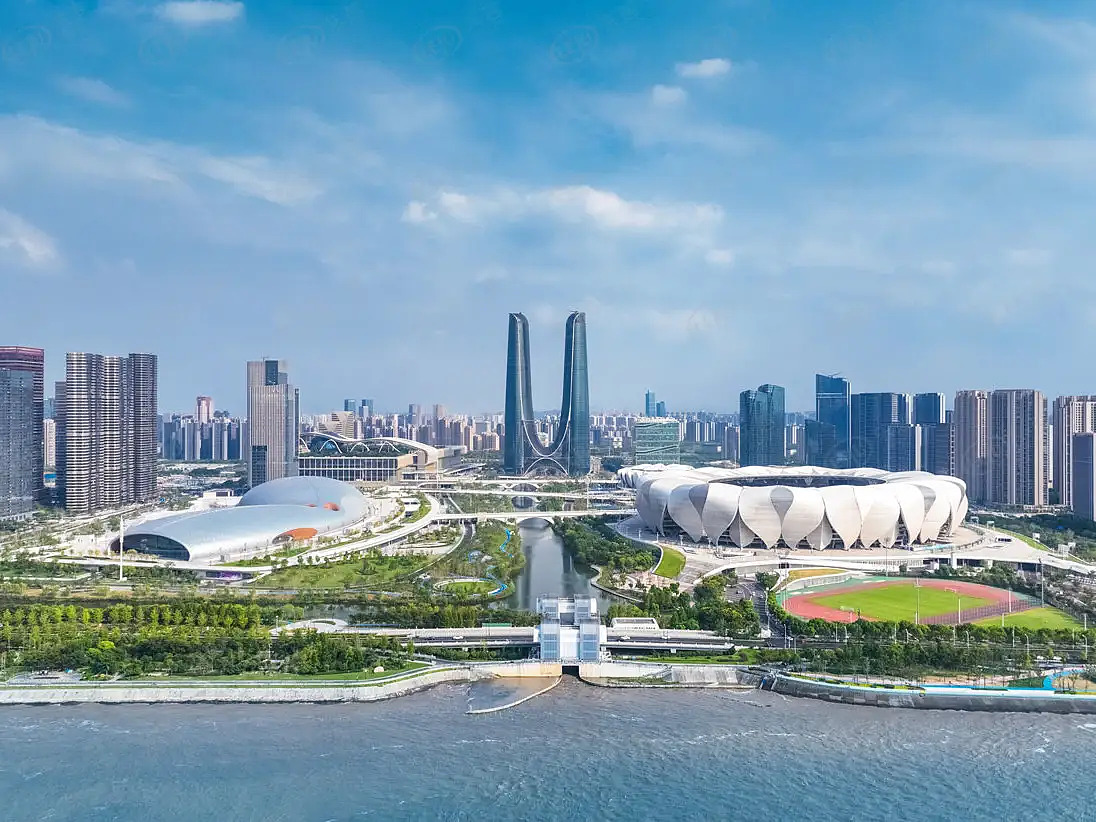
\includegraphics[width=\textwidth,clip,trim=0pt 2cm 0pt 8cm,]{hangzhou-arch.jpg}\\
图来自 \url{https://www.sohu.com/a/717899399_220260}
\end{block}


\begin{block}{\refname}
\renewcommand*{\bibfont}{\small\linespread{1}\selectfont}
\setlength{\biblabelsep}{0.25em}
\printbibliography[heading=none]
\end{block}

\end{frame}
\end{document}
